\chapter{UX e UI di prodotti interconnessi}

Quando ci si trova di fronte al compito di progettare l'interfaccia di un \textbf{dispositivo
	connesso}, si tende si tende ad adottare un approccio in linea alla \textit{vecchia
	scuola} della UI e UX. Si tende quindi a dare maggior peso e a spendere maggior concentrazione su aspetti come l'estetica delle interfacce e la forma del prodotto fisico. \textbf{Per l'IoT ciò non basta}.

Un prodotto interconnesso può avere un'ottima UI ma una pessima UX, esso non è costituito solamente dalla sua apparenza o dalla sua interfaccia, ma è \textbf{l'insieme delle due cose}.

Internet è un \textbf{mezzo di comunicazione}, fatto dagli uomini per gli uomini, \textbf{l'Internet of Things o IoT è un sistema di dispositivi informatici interconnessi}, macchine meccaniche o digitali \textbf{fornite di un identificatore unico detto UID}.

Esse possiedono la capacità di trasferire i dati sulla rete senza richiedere l'interazione uomo-uomo o uomo-computer.
La differenza tra i due mondi è sottile e spesso gli oggetti IoT sono creati per comunicare perfettamente tra di loro, ma hanno una pessima UI per l'uso umano, e
di conseguenza sono portatori di una pessima UX.

\section{Industry 4.0}

Il termine \textbf{Industria 4.0} indica l'ultima fase del processo con cui l'automazione industriale \textbf{integra} nuove \textbf{tecnologie produttive} per \textbf{migliorare} le condizioni di lavoro, creare nuovi modelli di business e aumentare la produttività e la qualità produttiva degli impianti.

I sistemi computerizzati monitorano i processi fisici, creando copie virtuali del mondo su cui sono basate le scelte e le decisioni future per il business dell'azienda.

\begin{figure}[!h]
	\centering
	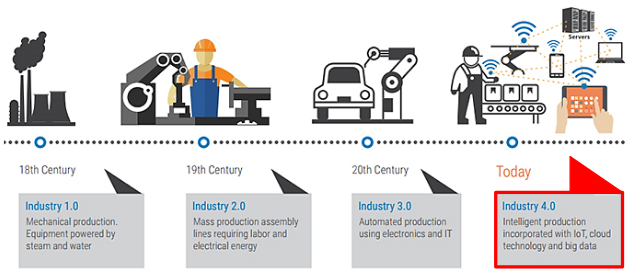
\includegraphics[scale=0.7]{immagini/Industry4.png}
\end{figure}

\pagebreak

Il problema di ogni tappa della rivoluzione industriale risiede nell'aumento esponenziale della \textbf{complessità informatica}. I dati parlano chiaro: il salto informativo dall'industria 3.0 all'industria 4.0 è pari al totale del salto effettuato da quando si usava l'asino come mezzo di locomozione fino alle attuali tecnologie.

\begin{figure}[!h]
	\centering
	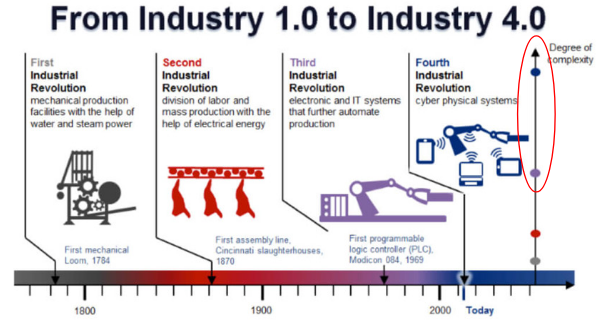
\includegraphics[scale=0.6]{immagini/Revolution.png}
\end{figure}

Quello che prima era un \textbf{processo produttivo}, con l'industria 4.0 diventa un \textbf{servizio} e la quantità di informazione necessaria cresce incredibilmente, di conseguenza progettare per la UX diventa estremamente complesso.

Ma come mai è importante questa evoluzione? Per le seguenti ragioni:

\begin{itemize}
	\item  Ottimizzando la produzione i profitti aumentano.
	\item Sarà possibile creare \textbf{nuovi modelli di business}.
	\item Saranno accessibili \textbf{nuove tecnologie}.
	\item Sarà possibile trasformare la forza lavoro: da operai in tecnici, capaci di estrarre informazioni dalle macchine e modificare la produzione di conseguenza.
\end{itemize}

Il cuore di un sistema interconnesso, sia di tipo consumer che industriale, è il
\textbf{Digital Twin}. Il \textbf{Digital Twin} è  \textbf{una copia digitale di un bene, di una macchina o di un processo reale esistente}. La comunicazione tra l'oggetto fisico e il Digital Twin è \textbf{continua e bidirezionale}. Tale strumento può essere usato sia per logging che per controllo remoto, ma sopratutto, è utile per simulazioni e manutenzione.

\begin{figure}[!h]
	\centering
	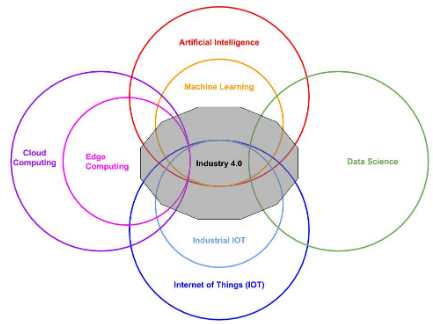
\includegraphics[scale=0.55]{immagini/Holistic.png}
\end{figure}

\pagebreak


\section{Products and Services in the 4.0 era}

\begin{figure}[!h]
	\centering
	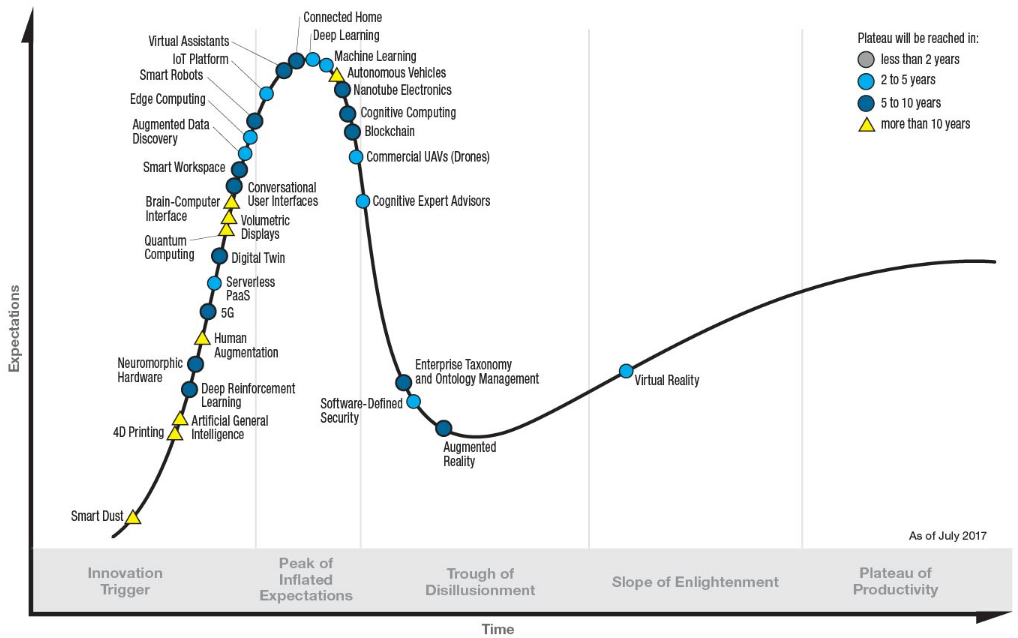
\includegraphics[scale=0.45]{immagini/Hype.png}
	\caption{Gartner Hype Cycle for emerging technologies.}
\end{figure}

L'IoT è solo una tecnologia abilitante, quindi non bisogna progettare per l'IoT bensì bisogna progettare sistemi interconnessi. Ciò altera il paradigma di progettazione: prima erano i computer ad essere dei centri di aggregazione tecnologica: qualche anno fa, ad esempio, in una qualsiasi casa, l'unico oggetto definibile smart era un \textbf{computer}, adesso si hanno più dispositivi connessi per svolgere svariate attività.

Sta sempre più emergendo il concetto di \textbf{intelligenza distribuita} accompagnata da un'\textbf{interfaccia personale}.

I dispositivi che si vuol progettare dovrebbero avere funzionalità altamente \textbf{specifiche} ma veicolate attraverso interfacce \textbf{generiche}. Le interfacce specifiche sono da evitare.

Si prenda, per esempio, un robot da cucina che riesce a fare
di tutto: frullare, centrifugare e cuocere, più una vasta gamma di funzionalità selezionabili, tramite pulsanti, uno per ogni funzione, attraverso un'interfaccia posta sul robot stesso. \textbf{Ciò è da ripudiare} in favore di un robot senza un singolo tasto che capisce da sè cosa va fatto e come farlo.

La progettazione per l'IoT è intrinsecamente più \textbf{complessa} della progettazione di servizi Web. Il design fisico, il design della UX e l'interconnettività di un unico sistema \textbf{non} possono essere gestiti separatamente.

I prodotti connessi pongono i progettisti dinanzi a sfide progettuali nuove, molte delle quali derivano da:

\begin{itemize}
	\item La \textbf{natura} specializzata dei servizi \textbf{IoT}.
	\item La capacità dei dispositivi IoT di fare da \textbf{ponte tra il mondo digitale e fisico}.
	\item Il fatto che molti prodotti IoT siano \textbf{sistemi distribuiti composti da più dispositivi}.
	\item \textbf{Le stranezze del networking}.
\end{itemize}

\pagebreak

\section{Real world context}
Le interfacce, nel mondo dell'IoT, sono sensori e attuatori. I \textbf{sensori} convertono una variabile \textbf{fisica} in un segnale \textbf{elettrico}, mentre gli
attuatori convertono un segnale\textbf{ elettrico} in una variabile \textbf{fisica}.

Gli attuatori possono essere controllati a distanza o automatizzati, ma a differenza dei comandi digitali, le azioni sul mondo reale \textbf{non possono essere annullate}.
Questo contesto fisico di utilizzo crea ulteriori sfide. Nell'IoT non si può dare per
scontato lo stato d'animo dell'utente mentre interagisce con l'oggetto.

Gli oggetti ubiquitari, andando a posizionarsi nei vari angoli della casa o dell'ufficio, si trovano ad interagire con persone che potrebbero momentaneamente \textbf{non essere predisposte all'interazione con un oggetto digitale}, ciò rende l'errore molto più frequente.

Si devono creare quindi oggetti molto semplici sia da capire che da utilizzare.

Un altro aspetto importante è l'\textbf{interusabilità}, cioè la proprietà del sistema di essere usato attraverso \textbf{tutti} i dispositivi o le interfacce che lo compongono (\textit{e.g. Google Assistant può essere usato tramite app, sito web o Google Home}).

\begin{figure}[!h]
	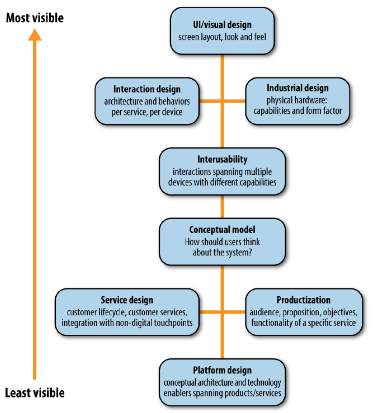
\includegraphics[scale=0.55]{immagini/UX_IoT.png}
	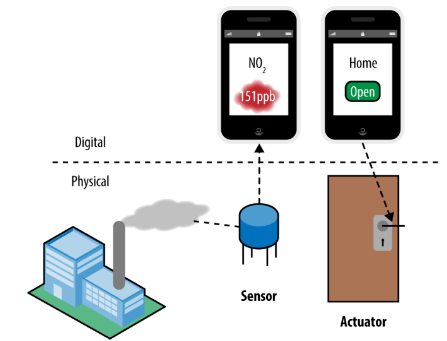
\includegraphics[scale=0.5]{immagini/Sensors_actuators.png}
\end{figure}

\begin{flushleft}
	\textit{Perché puntare così tanto su
		questa caratteristica?}
\end{flushleft}

Bisogna infatti consentire all'utente l'accesso e l'interazione col sistema dove e come egli la desidera, il più compatibilmente possibile con le circostanze in cui egli si trova. L'\textbf{esperienza} dell'utente \textbf{non deve però differire} tra le varie interfacce. Inoltre, gli utenti hanno bisogno di una certa comprensione di come funziona il sistema. Anche i prodotti connessi piuttosto semplici sono concettualmente molto più complessi di quelli non connessi. Quindi è necessario un oggetto che veicoli un modello \textbf{concettuale chiaro}, in modo tale che l'utente si crei un modello mentale solido.

È necessario quindi creare un
\textbf{modello unificato di interazione}, dove è chiaro che l'interfaccia e l'intelligenza sono distribuite, in modo tale da veicolare all'utente un \textbf{unico} modello concettuale utilizzabile per l'intero sistema.

Un'altra problematica è che molti progettisti progettano supponendo che i dispositivi siano sempre connessi, ma questo \textbf{non è sempre vero}! Anzi conviene rovesciare il paradigma, \textbf{progettando per l'assenza di internet e assumendo che sia disponibile solo sporadicamente}. Con questo modo di progettare si considerano anche i ritardi e i problemi dovuti alle reti fisiche e alla trasmissione su di esse.

